\section{The Cylindrical Helix}\label{sec:geometry}
This section presents the basic definitions and equations which describe the geometry of a monofilar thin wire helix which will be utilized in the sheath-helix field derivations. 
\subsection{Basic Geometry}\label{subsec:basicGeometry}
The basic geometry of a helix is shown in Fig. \ref{fig:helix}. Here, $\delta$ represents the width of the `tape' helix while $a$, $p$, and $\psi$ represent the helix radius, turn-to-turn pitch, and pitch angle, respectively. For a monofilar helix with infinitesimally thin wire, we take $\delta\rightarrow0$, effectively neglecting the `tape' nature of the structure or the finite thickness of the conductor comprising the helix. The pitch angle of the helix is defined as
\begin{equation}\label{eq:pitchAngle}
	\psi = \tan^{-1}\left(\frac{p}{2\pi r}\right)
\end{equation}

\begin{figure}[b]
	\centering
	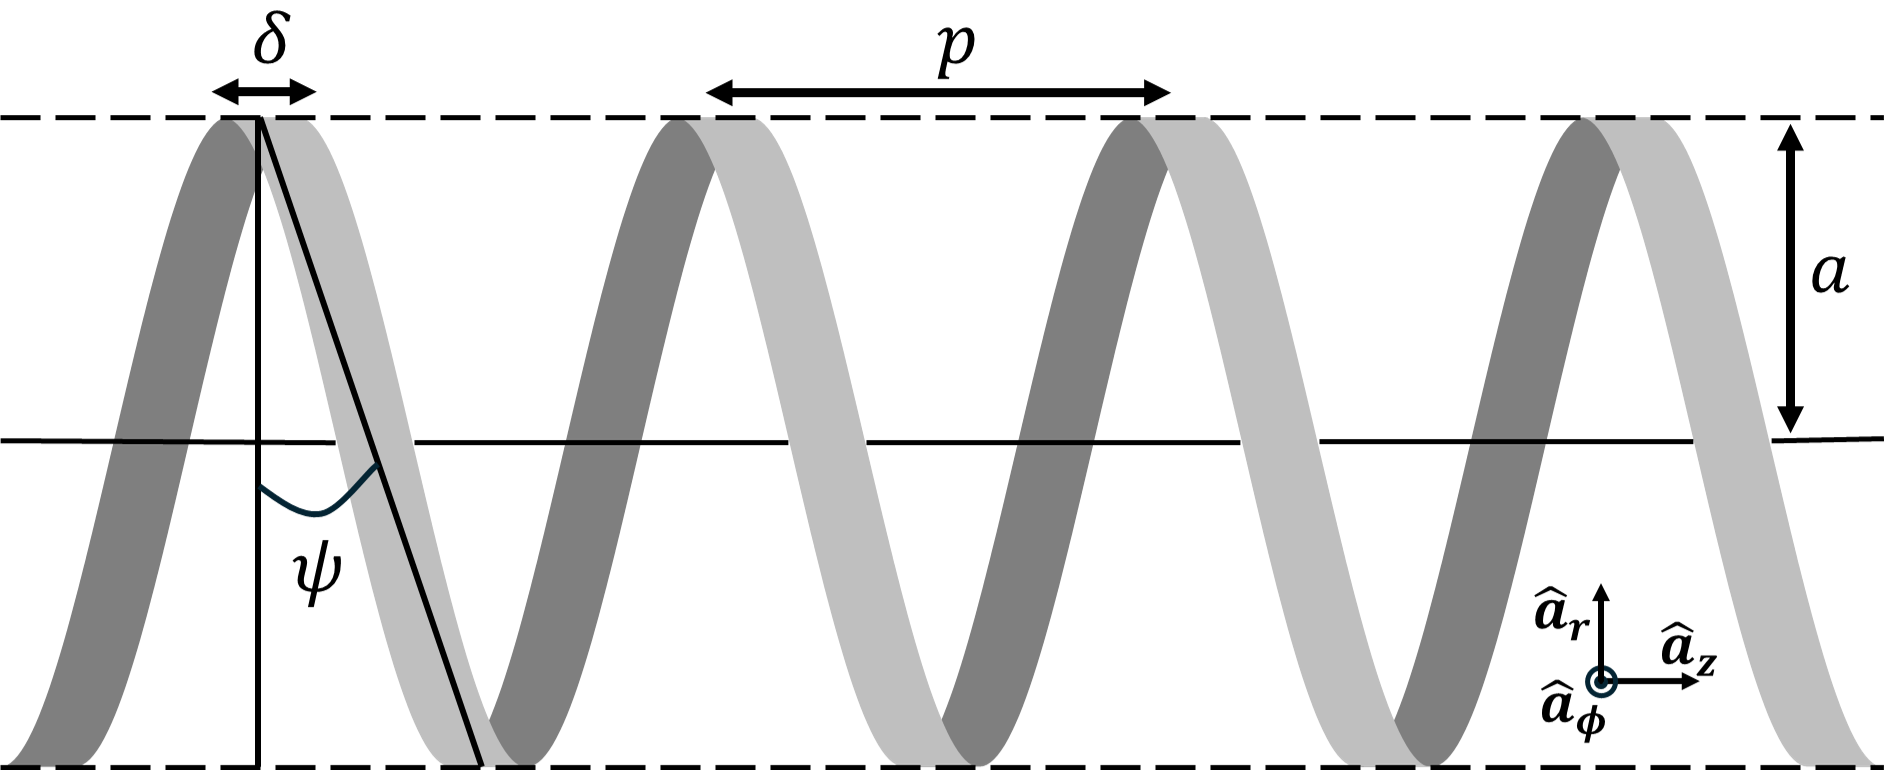
\includegraphics[width=\textwidth]{helix}
	\caption{Helix geometry.}
	\label{fig:helix}
\end{figure}
If the helix has $N$ turns, the total length of the structure is $L=Np$. However, the total arc length of each turn is found as $L_n = \sqrt{p^2 + (2\pi a)^2}$ such that the total path length of the helical conductor is 
\begin{equation}
	L_h = N\sqrt{p^2 + (2\pi a)^2}
\end{equation}

The parametric equations defining the circular helical position vector $\vec{R}$ can be written in terms of the azimuthal angle $\phi$ as 
\begin{equation}\label{eq:parametric}
	\vec{\mathbf{R}}(\phi) = \left\langle x(\phi), y(\phi), z(\phi) \right\rangle = \left\langle a\cos(\phi), a\sin(\phi), \frac{p}{2\pi}\phi \right\rangle
\end{equation}

\subsection{Helical Unit Vectors}
To solve the boundary value problem of the sheath helix, it will be necessary to subject the wave equations to the helical boundary conditions. These boundary conditions require evaluation of the tangential and normal field components across the helical conductor. It is therefore necessary to develop unit vectors which are both parallel and perpendicular to the helical axis. The tangent vector $\vec{\mathbf{T}}$ along the helical direction is found from the position vector in (\ref{eq:parametric}) as
\begin{equation}\label{eq:tangent}
	\vec{\mathbf{T}} = \frac{d\vec{\mathbf{R}}}{d\phi} = -a\sin(\phi)\hat{\mathbf{a}}_{x} + a\cos(\phi)\hat{\mathbf{a}}_{y} + \frac{p}{2\pi}\hat{\mathbf{a}}_{z}
\end{equation}
Recognizing the bases vector transformation $\hat{\mathbf{a}}_{\phi} = -\sin(\phi)\hat{\mathbf{a}}_{x}+\cos(\phi)\hat{\mathbf{a}}_{y}$, (\ref{eq:tangent}) can be rewritten as
\begin{equation}\label{eq:tangentRad}
	\vec{\mathbf{T}} = a{\mathbf{a}}_{\phi} + \frac{p}{2\pi}\hat{\mathbf{a}}_{z}
\end{equation}
The magnitude of (\ref{eq:tangentRad}) is 
\begin{equation}\label{eq:tangentMag}
	|\vec{\mathbf{T}}| = \sqrt{a^2 + \left(\frac{p}{2\pi}\right)^2}
\end{equation}
The unit tangent vector $\hat{\mathbf{a}}_{T}$ is then
\begin{equation}\label{eq:tangentUnit}
	\hat{\mathbf{a}}_{T} = \frac{\vec{\mathbf{T}}}{|\vec{\mathbf{T}}|} 
	= \frac{a}{\sqrt{a^2 + \left(\frac{p}{2\pi}\right)^2}} \mathbf{a}_{\phi} 
	+ \frac{p}{2\pi\sqrt{a^2 + \left(\frac{p}{2\pi}\right)^2}} \mathbf{a}_{z}
\end{equation}
Now, the definition of the pitch angle in (\ref{eq:pitchAngle}) mathematically corresponds to the right triangle shown in Fig. \ref{fig:triangle}.
\begin{figure}[h]
	\centering
	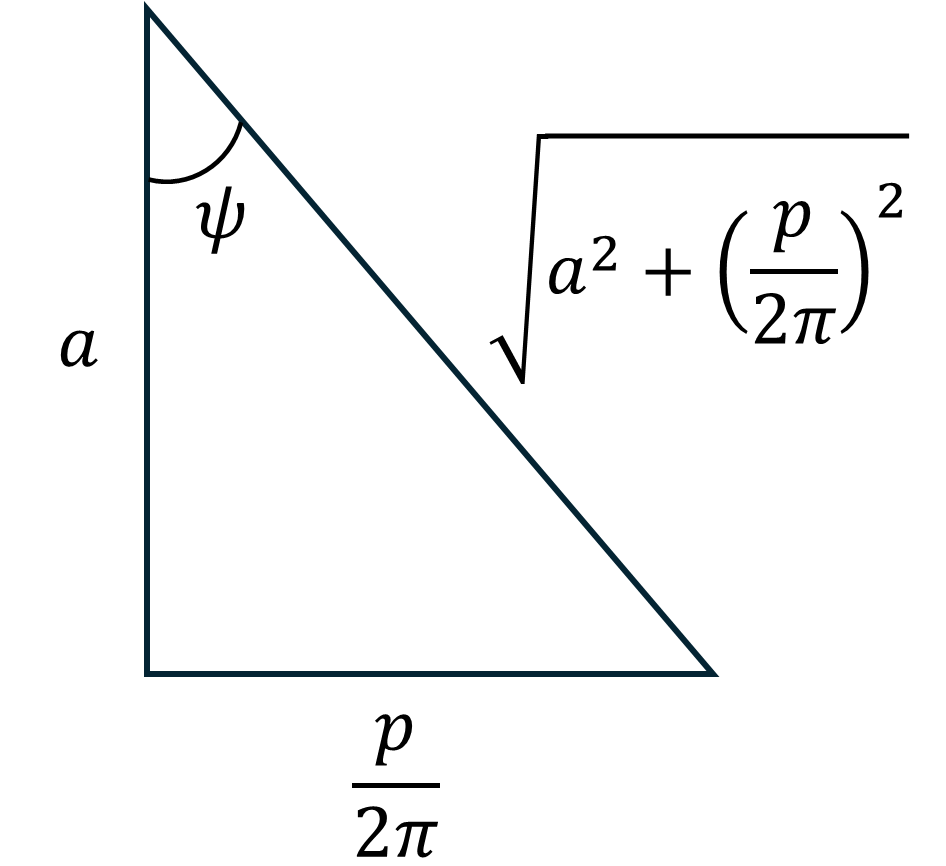
\includegraphics[width=0.3\textwidth]{triangle}
	\caption{Equivalent right triangle for pitch angle definition.}
	\label{fig:triangle}
\end{figure}

The following relationships then hold
\begin{equation}\label{eq:tangenCos}
	\cos(\psi) = \frac{a}{\sqrt{a^2 + \left(\frac{p}{2\pi}\right)^2}}
\end{equation}
\begin{equation}\label{eq:tangentSin}
	\sin(\psi) = \frac{p}{2\pi\sqrt{a^2 + \left(\frac{p}{2\pi}\right)^2}}
\end{equation}
Plugging (\ref{eq:tangenCos}) and (\ref{eq:tangentSin}) into (\ref{eq:tangentUnit}) finally gives (\ref{eq:parallel}), the unit vector parallel to the helical conductor. 
\begin{equation}\label{eq:parallel}
	\hat{\mathbf{a}}_{\parallel} =  \cos(\psi)\mathbf{a}_{\phi} 
	+ \sin(\psi)\mathbf{a}_{z}
\end{equation}
The unit vector perpendicular to the conductor is then
\begin{equation}\label{eq:perpendicular}
	\hat{\mathbf{a}}_{\perp} =  \hat{\mathbf{a}}_{r} \times \hat{\mathbf{a}}_{\parallel} = -\sin(\psi)\mathbf{a}_{\phi} + \cos(\psi)\mathbf{a}_{z}
\end{equation}
(\ref{eq:parallel}) and (\ref{eq:perpendicular}) can then be used to enforce the electromagnetic boundary conditions on the tangential and normal components of the electric and magnetic fields at helical boundaries of interest.